%------------------------------------------------------------------------------
% Template file for the submission of papers to IUCr journals in LaTeX2e
% using the iucr document class
% Copyright 1999-2013 International Union of Crystallography
% Version 1.6 (28 March 2013)
%------------------------------------------------------------------------------

\documentclass[]{setup/iucr}              % DO NOT DELETE THIS LINE

     %-------------------------------------------------------------------------
     % Information about journal to which submitted
     %-------------------------------------------------------------------------
     \journalcode{E}              % Indicate the journal to which submitted
                                  %   A - Acta Crystallographica Section A
                                  %   B - Acta Crystallographica Section B
                                  %   C - Acta Crystallographica Section C
                                  %   D - Acta Crystallographica Section D
                                  %   E - Acta Crystallographica Section E
                                  %   F - Acta Crystallographica Section F
                                  %   J - Journal of Applied Crystallography
                                  %   M - IUCrJ
                                  %   S - Journal of Synchrotron Radiation
% \documentclass[twocolumn]{article}
%%%%%%%%%%%%%%%%%%%%%%%%%%%%%%%%%%%%%%%%%%%%%%%%
% Encoding and fonts
%%%%%%%%%%%%%%%%%%%%%%%%%%%%%%%%%%%%%%%%%%%%%%%%
% Choose the output font encoding
\usepackage[T1]{fontenc}
% Choose the input encoding (how your source files are encoded)
\usepackage[utf8]{inputenc}

% Use the vector font Latin Modern which is going
% to be the default font in latex in the future.
% \usepackage{lmodern}
% \pdfmapfile{ua1r8r.map}

% Make latex understand and use the typographic
% rules of the language used in the document.
\usepackage[english, french]{babel}

%%%%%%%%%%%%%%%%%%%%%%%%%%%%%%%%%%%%%%%%%%%%%%%%
% Graphics (images, tables, ...)
%%%%%%%%%%%%%%%%%%%%%%%%%%%%%%%%%%%%%%%%%%%%%%%%

% Figures - TIKZ (Build figures inside LaTeX)
\usepackage{tikz}
\usetikzlibrary{arrows,shapes,positioning,shadows,trees}

%%%%%%%%%%%%%%%%%%%%%%%%%%%%%%%%%%%%%%%%%%%%%%%%
% Mathematics
%%%%%%%%%%%%%%%%%%%%%%%%%%%%%%%%%%%%%%%%%%%%%%%%
% Defines new environments such as equation,
% align and split 
% Provides additional features to amsmath
\usepackage[intlimits]{mathtools}
\usepackage{relsize}
% Adds new math symbols
\usepackage{amssymb}

% Use theorems in your document
% The ntheorem package is also used for the example environment
% When using thmmarks, amsmath must be an option as well. Otherwise \eqref doesn't work anymore.
\usepackage[framed,amsmath,thmmarks]{ntheorem}

%%%%%%%%%%%%%%%%%%%%%%%%%%%%%%%%%%%%%%%%%%%%%%%%
% Physics and chemistry
%%%%%%%%%%%%%%%%%%%%%%%%%%%%%%%%%%%%%%%%%%%%%%%%
% Provide SI units macros, to use proper formatting that respects SI standards
\usepackage{siunitx}
\sisetup{decimalsymbol=comma}
\sisetup{binary-units}
\sisetup{detect-weight}
\sisetup{inter-unit-product=\ensuremath{{} \cdot {}}}
\usepackage{cancel}

\usepackage[version=4]{mhchem}

% Macros are defined in setup/macros.tex

%%%%%%%%%%%%%%%%%%%%%%%%%%%%%%%%%%%%%%%%%%%%%%%%
% Misc
%%%%%%%%%%%%%%%%%%%%%%%%%%%%%%%%%%%%%%%%%%%%%%%%

% Enables the use FiXme refferences. Syntax: \fxnote{...} %%%
% When the document is in "final" version instead of "draft",
% an error will occur for every FiXme under compilation.
\usepackage[french, silent]{fixme}
\fxusetheme{color}
\fxsetup{layout=marginclue,footnote}
 % Packages inclusion
%%%%%%%%%%%%%%%%%%%%%%%%%%%%%%%%%%%%%%%%%%%%%%%%%%%%%
%             UNITS, EQUATIONS AND TEXT             %
%%%%%%%%%%%%%%%%%%%%%%%%%%%%%%%%%%%%%%%%%%%%%%%%%%%%%

\newcommand{\eq}[2]{\si{#1} &= \si{#2}}
\newcommand{\iaoi}{&& &\Updownarrow&&}  % 'If and only if' sign printed vertically between two equations
\newcommand{\eqOne}[2]{\si{#1} &= \si{#2} &\nonumber\\}
\newcommand{\eqTwo}[1]{&\ \ \ \ \si{#1}&}
% Text:
\newcommand{\tx}[1]{\text{#1}}
\newcommand{\deriv}{\mathrm{d}}

\newcommand{\noun}[1]{\textsc{#1}}
\newcommand*{\rom}[1]{\expandafter\@slowromancap\romannumeral #1@}

% Matrices, vectors & quaternions
%\renewcommand{\vec}[1]{\boldsymbol{\bf{#1}}}
\newcommand{\mat}[1]{#1}
\newcommand{\quat}[1]{\boldsymbol{\mathbf{#1}}}
\newcommand{\quatprod}{\otimes}

% Useful for declaration of math terms signification, right after an equation
\renewcommand*\descriptionlabel[1]{\hspace\leftmargin$#1$}

% Vertical line in equations ie. |_x=y (whereTwo stacks two equalities at the line)
\newcommand{\where}[1]{ \left.\rule{0cm}{.5cm}\right\vert\rule{0cm}{.4cm}_{\substack{\rule{0cm}{.15cm}\\ \si{#1} }} }
\newcommand{\whereTwo}[2]{ \left.\rule{0cm}{.67cm}\right\vert\rule{0cm}{.5cm}_{\substack{\si{#1} \rule{0cm}{.19cm}\\\vspace{-.1cm}\\ \si{#2}}} }

\newcommand{\sample}[1]{\ensuremath{#1}}

\makeatletter
  % Reaction equations environments
  \newcommand\reaction@[1]{\begin{equation}\ce{#1}\end{equation}}
  \newcommand\reaction@nonumber[1]{\begin{equation*}\ce{#1}\end{equation*}}
  \newcommand\reaction{\@ifstar{\reaction@nonumber}{\reaction@}}

  % Layer stacks and redox couples, useful in physics
  \newcommand*\stackslash{\text{/}\allowbreak}
  \newcommand*\stackhyphen{\text{-}\allowbreak}
  \newcommand*\stackpipe{\text{|}\allowbreak}
  \newcommand\stack[1]{%
    \cesplit{%
      {\/}{\c{stackslash}}%
      {-}{\c{stackhyphen}}%
      {\|}{\ \c{stackpipe}\ }%
    }{#1}%
  }
  \newcommand*\dopingcolumn{\text{:}\allowbreak}
  \newcommand\doped[1]{%
    \cesplit{%
      {:}{\c{dopingcolumn}}%
    }{#1}%
  }
\makeatother

% Hermann-Mauguin notation (for cristallographic symmetries)
\newcommand{\hmn}[1]{% Hermann-Maguin notation
  \ensuremath{\begingroup\setupHMN #1\endgroup}%
}

\newcommand{\setupHMN}{%
  \doHMN{-}{\HMNoverline}%
  \doHMN{*}{\HMNminverse}%
  \doHMN{i}{\infty}
}

\newcommand{\doHMN}[2]{%
  \begingroup\lccode`~=`#1
  \lowercase{\endgroup\let~}#2%
  \mathcode`#1="8000
}

\newcommand{\HMNminverse}[1]{\frac{#1}{m}}
\newcommand{\HMNoverline}[1]{\mkern1mu\overline{\mkern-1mu#1\mkern-1mu}\mkern1mu}


% \ExplSyntaxOn
% \NewDocumentCommand{\hmn}{m}
%  {
%   \ensuremath
%    {
%     \hermannmauguin_group:n { #1 }
%    }
%  }

% \tl_new:N \l_hermannmauguin_input_tl
% \tl_new:N \l_hermannmauguin_output_tl

% \cs_new_protected:Nn \hermannmauguin_group:n
%  {
%   \tl_set:Nn \l_hermannmauguin_input_tl { #1 }
%   \tl_clear:N \l_hermannmauguin_output_tl
%   \tl_map_inline:Nn \l_hermannmauguin_input_tl
%    {
%     \__hermannmauguin_item:n { ##1 }
%    }
%   \! % kill the first \,
%   \tl_use:N \l_hermannmauguin_output_tl
%  }

% \cs_new_protected:Nn \__hermannmauguin_item:n
%  {
%   \str_case:nnF { #1 }
%    {
%     {*}{ \__hermannmauguin_put:n { \__hermannmauguin_inverse:Nn } }
%     {-}{ \__hermannmauguin_put:n { \__hermannmauguin_overline:Nn } }
%     {i}{ \__hermannmauguin_put:n { \,\infty } }
%    }
%    { \__hermannmauguin_put:n { \, {#1} } }
%  }

% \cs_new_protected:Nn \__hermannmauguin_put:n
%  {
%   \tl_put_right:Nn \l_hermannmauguin_output_tl { #1 }
%  }

% \cs_new_protected:Nn \__hermannmauguin_overline:Nn
%  {% #1 should be \,; #2 is the number to operate on
%   #1 \mkern1mu\overline{\mkern-1mu#2\mkern-1mu}\mkern1mu
%  }
% \cs_new_protected:Nn \__hermannmauguin_inverse:Nn
%  {% #1 should be \,; #2 is the number to operate on
%   #1 \frac{ #2 } { m }
%  }
% \ExplSyntaxOff

%%%%%%%%%%%%%%%%%%%%%%%%%%%%%%%%%%%%%%%%%%%%%%%%%%%%%
%                 TIKZ SETTINGS                     %
%%%%%%%%%%%%%%%%%%%%%%%%%%%%%%%%%%%%%%%%%%%%%%%%%%%%%
\usetikzlibrary{arrows.meta}
\tikzset{
  block/.style  = {draw, thick, rectangle,
                     minimum height = 2.1em,
                     minimum width = 1.7em},
  sum/.style    = {draw, circle, inner sep=1.5pt},
  basic/.style  = {draw, text width=190pt, minimum height=45pt,
                   font=\sffamily, inner sep=0pt},
}

% Node macro to build trees
\newcommand\mynode[5][]{
  \node[#1] (#2)
  {\parbox{20pt}{%
      \includegraphics[width=45pt]{#3}}%
    \parbox{25pt}{\mbox{}}%  
    \parbox{\dimexpr190pt-30pt\relax}{#4\\[.4ex]#5}%
  };
}

%%%%%%%%%%%%%%%%%%%%%%%%%%%%%%%%%%%%%%%%%%%%%%%%%%%%%
%                  REFERENCES                       %
%%%%%%%%%%%%%%%%%%%%%%%%%%%%%%%%%%%%%%%%%%%%%%%%%%%%%

%Chapter
\newcommand{\Chapref}[1]{\emph{Chapitre \ref{#1}}}
\newcommand{\chapref}[1]{\emph{chapitre \ref{#1}}}
%Section
\newcommand{\Secref}[1]{\emph{Section \ref{#1}}}
\newcommand{\secref}[1]{\emph{section \ref{#1}}}
%subSection
\newcommand{\Subsecref}[1]{\emph{Sous-section \ref{#1}}}
\newcommand{\subsecref}[1]{\emph{sous-section \ref{#1}}}
%Appendix
\newcommand{\Appref}[1]{\emph{Annexe \ref{#1}}}
\newcommand{\appref}[1]{\emph{annexe \ref{#1}}}
%Listings
\newcommand{\Coderef}[1]{\emph{Listing: \ref{#1}}}
\newcommand{\coderef}[1]{\emph{listing: \ref{#1}}}
%Figure:
\newcommand{\Figref}[1]{\emph{Figure \ref{#1}}}
\newcommand{\figref}[1]{\emph{figure \ref{#1}}}
\newcommand{\FigrefTwo}[2]{\emph{Figures \ref{#1}} et \emph{\ref{#2}}}
\newcommand{\figrefTwo}[2]{\emph{figures \ref{#1}} et \emph{\ref{#2}}}
%Table:
\newcommand{\Tableref}[1]{\emph{Table \ref{#1}}}
\newcommand{\tableref}[1]{\emph{table \ref{#1}}}

%Expressions:
\newcommand{\Expr}[1]{\emph{Expression (\ref{#1})}}
\newcommand{\expr}[1]{\emph{expression (\ref{#1})}}

%Equations:
%1 equation:
\newcommand{\Eqref}[1]{\emph{Équation (\ref{#1})}}
\renewcommand{\eqref}[1]{\emph{équation (\ref{#1})}}
%2 equations:
\newcommand{\EqrefTwo}[2]{\emph{Équations (\ref{#1})} et \emph{(\ref{#2})}}
\newcommand{\eqrefTwo}[2]{\emph{équations (\ref{#1})} et \emph{(\ref{#2})}}
%3 equations:
\newcommand{\EqrefThree}[3]{\emph{Equation (\ref{#1})}, \emph{(\ref{#2})} and \emph{(\ref{#3})}}
\newcommand{\eqrefThree}[3]{\emph{equation (\ref{#1})}, \emph{(\ref{#2})} and \emph{(\ref{#3})}}
%4 equations:
\newcommand{\EqrefFour}[4]{\emph{Equation (\ref{#1})}, \emph{(\ref{#2})}, \emph{(\ref{#3})} and \emph{(\ref{#4})}}
\newcommand{\eqrefFour}[4]{\emph{equation (\ref{#1})}, \emph{(\ref{#2})}, \emph{(\ref{#3})} and \emph{(\ref{#4})}}
%5 equations:
\newcommand{\EqrefFive}[5]{\emph{Equation (\ref{#1})}, \emph{(\ref{#2})}, \emph{(\ref{#3})}, \emph{(\ref{#4})} and \emph{(\ref{#5})}}
\newcommand{\eqrefFive}[5]{\emph{equation (\ref{#1})}, \emph{(\ref{#2})}, \emph{(\ref{#3})}, \emph{(\ref{#4})} and \emph{(\ref{#5})}}
%6 equations:
\newcommand{\EqrefSix}[6]{\emph{Equation (\ref{#1})}, \emph{(\ref{#2})}, \emph{(\ref{#3})}, \emph{(\ref{#4})}, \emph{(\ref{#5})} and \emph{(\ref{#6})}}
\newcommand{\eqrefSix}[6]{\emph{equation (\ref{#1})}, \emph{(\ref{#2})}, \emph{(\ref{#3})}, \emph{(\ref{#4})}, \emph{(\ref{#5})} and \emph{(\ref{#6})}}
%7 equations:
\newcommand{\EqrefSeven}[7]{\emph{Equation (\ref{#1})}, \emph{(\ref{#2})}, \emph{(\ref{#3})}, \emph{(\ref{#4})}, \emph{(\ref{#5})}, \emph{(\ref{#6})} and \emph{(\ref{#7})}}
\newcommand{\eqrefSeven}[7]{\emph{equation (\ref{#1})}, \emph{(\ref{#2})}, \emph{(\ref{#3})}, \emph{(\ref{#4})}, \emph{(\ref{#5})}, \emph{(\ref{#6})} and \emph{(\ref{#7})}} % My new macros

\begin{document}                  % DO NOT DELETE THIS LINE

     %-------------------------------------------------------------------------
     % The introductory (header) part of the paper
     %-------------------------------------------------------------------------

     % The title of the paper. Use \shorttitle to indicate an abbreviated title
     % for use in running heads (you will need to uncomment it).

\title{Redétermination de la structure cristallographique de la pyrite (\ce{FeS2})}
%\shorttitle{Short Title}

     % Authors' names and addresses. Use \cauthor for the main (contact) author.
     % Use \author for all other authors. Use \aff for authors' affiliations.
     % Use lower-case letters in square brackets to link authors to their
     % affiliations; if there is only one affiliation address, remove the [a].

\cauthor{Julien}{Bréhin}{julien.brehin@etu.upmc.fr}{}
\author{Mourad}{Mezaguer}

\aff{M2 Sciences des Matériaux et Nano-Objets, Sorbonne Université, Paris, FRANCE}

     % Use \shortauthor to indicate an abbreviated author list for use in
     % running heads (you will need to uncomment it).

%\shortauthor{Soape, Author and Doe}

     % Use \vita if required to give biographical details (for authors of
     % invited review papers only). Uncomment it.

%\vita{Author's biography}

     % Keywords (required for Journal of Synchrotron Radiation only)
     % Use the \keyword macro for each word or phrase, e.g. 
     % \keyword{X-ray diffraction}\keyword{muscle}

%\keyword{keyword}

     % PDB and NDB reference codes for structures referenced in the article and
     % deposited with the Protein Data Bank and Nucleic Acids Database (Acta
     % Crystallographica Section D). Repeat for each separate structure e.g
     % \PDBref[dethiobiotin synthetase]{1byi} \NDBref[d(G$_4$CGC$_4$)]{ad0002}

%\PDBref[optional name]{refcode}
%\NDBref[optional name]{refcode}

\maketitle                        % DO NOT DELETE THIS LINE

\begin{abstract}
Dans cet article, on s'attèle à étudier un minéral ayant une notoriété historique, à savoir la pyrite (\ce{FeS2}), aussi nommé «or des fous».\\
L'objectif est de re-déterminer ses symétries et sa structure par analyse macroscopique de monocristaux complémentée par des expériences de diffraction des rayons X.
Les méthodes de diffraction utilisées (méthode de Laue, en laboratoire, puis méthode des poudres sur la ligne CRISTAL du synchrotron SOLEIL) permettent de retrouver la classe de Laue et de remonter étape par étape jusqu'au groupe d'espace \hmn{Pa-3} de la pyrite.
Enfin, on donne les positions atomiques obtenues par essais et erreurs et on discute d'une méthode plus précise pour l'affinement des derniers paramètres cristallographiques.
\fxnote{Update abstract}
\end{abstract}


     %-------------------------------------------------------------------------
     % The main body of the paper
     %-------------------------------------------------------------------------
     % Now enter the text of the document in multiple \section's, \subsection's
     % and \subsubsection's as required.

\section{Introduction}

La pyrite, de formule chimique \ce{FeS2}, est plus connue sous le nom de «~pierre à feu~». Elle doit d'ailleurs son nom à sa capacité à produire des étincelles lorsqu'on la frotte ou qu'on la soumet à des chocs avec certains autres matériaux. Longtemps surnommée «~l'or des fous~» de par sa teinte et son aspect qui ont sûrement trompé plus d'un chercheur d'or, la pyrite est aujourd'hui particulièrement utilisée en joaillerie ou dans l'industrie chimique, pour la fabrication d'acide sulfurique. \fxnote{Citation needed}\\
On la trouve naturellement en quantités relativement abondantes dans des gisements à des endroits très divers, en Europe comme en Amérique (lieu d'une «~ruée vers l'or~» au XIXe siècle). Bien qu'elle soit souvent mélangée, par exemple à d'autres composés proches où le fer est substitué par d'autres métaux, il est également possible d'extraire des monocristaux de \ce{FeS2} de taille assez importante sous forme de cubes surprenamment très lisses ou de sous forme de pentagono-dodécaèdres.

La pyrite fait donc partie des minéraux que l'on connaît et que l'on a utilisé depuis assez longtemps pour ses propriétés macroscopiques, avant-même de comprendre ses propriétés mésoscopiques et \textit{a fortiori} nanoscopiques.\\
Dans cet article, on s'attachera à déterminer par des expériences de diffraction de rayons X, la structure cristallographique complète de la pyrite, en partant d'une étude macroscopique et jusqu'à retrouver son groupe d'espace et ses paramètres de maille.
% But de l'article : déterminer la structure cristallographique complète de la pyrite

\section{Analyse préalable des symétries}
% Étude préliminaire : Forme des monocristaux
% Éléments de symétrie et groupe ponctuel du cube
% Éléments de symétrie et groupe ponctuel du pentagono-dodécaèdre


\section{Méthodes expérimentales}
% Méthodes expérimentales DRX (Laue + SOLEIL/CRISTAL)

Une première expérience de diffraction de rayons X a été réalisée sur des dispositifs spécifiques présents au laboratoire IMPMC de Sorbonne Université, en utilisant la méthode de Laue en transmission (longueur d'onde polychromatique dans un certain intervalle, échantillon fixe pendant la mesure).\\
La source de rayons X utilisée était un tube à anticathode en cuivre dont la raie \(K_{\alpha_1,\ce{Cu}}\) est de longueur d'onde \(\lambda_{K_{\alpha_1,\ce{Cu}}}=\SI{0.1545}{\nano\metre}\) (la cathode en tungstène était excitée avec une tension de \SI{40}{\kilo\volt} et un courant de \SI{30}{\milli\ampere}). La lecture du cliché de diffraction de Laue a été réalisée à partir de films réutilisables photosensibles aux RX et numérisés après exposition avec un scanner du même constructeur.\fxnote{Trouver constructeur}\\
L'échantillon \textit{a priori} monocristallin placé entre la source et le détecteur était monté sur un support permettant un pivot autour de l'axe \hmn{[hkl]}\fxnote{Indiquer direction correcte}.

Une mesure de diffraction sur synchrotron a également été réalisée sur la ligne CRISTAL du synchrotron SOLEIL.\fxnote{Citer la ligne CRISTAL} La mesure a été effectuée sur un échantillon poudreux de pyrite (\ce{FeS2}) avec un diffractomètre 2 cercles et pour un longueur d'onde incidente monochromatique correspondant à une énergie \(E_i = \SI{17017}{\electronvolt}\), soit \(\lambda_i = \SI{0.07285}{\nano\metre}\).\\
% Le diffractogramme expérimental obtenu sur la \figref{fig:diffractogrammeSOLEIL} est analysé en \secref{sec:}

\section{Détermination du groupe de Laue}
% Observation des éléments de symétrie du cliché de Laue
% Détermination du groupe de Laue -> comparaison avec le groupe ponctuel supposé et limites des clichés de Laue
% => Diffractogramme sur synchrotron (justifications)

\section{Obtention du mode de réseau}
% Tableau des 10 premières raies : numéro des raies (h²+k²+l²), indices (hkl), angles 2*theta, d_hkl, d_i+1/d_i, paramètre de maille
% Lecture des positions angulaires (2*theta) des 10 premières raies
% Calcul des distances inter-réticulaires (Loi de Bragg)
% Calcul des valeurs de rapport entre distances inter-réticulaires (di+1/di)
% Intérêt de ces rapports et comparaison des valeurs expérimentales avec des rapports calculés
% Obtention des indices hkl pour chacune des raies et détermination du mode de réseau (primitif, sinon il y aurait plus d'extinctions -> facteur de structure décomposé en mode+motif)

\section{Calcul du paramètre de maille cubique}
% Détermination du paramètre de maille cubique à partir des d_hkl (formule)
% Moyenne et écart-type de a

\section{Détermination du groupe d'espace}
% Remarque sur le rapport à valeur étrange et explication sur la raie manquante
% Autres directions manquantes sur le diffractogramme
% Parité des directions manquantes et comparaison avec les IToC (annexe 3)
% Déduction du groupe d'espace
% Explication extinctions élément de symétrie (élément translatoire => facteur de structure)

\section{Conclusion}
% Positions atomiques (motif), sites de Wyckoff, ...
% Modèle VESTA
% Comparaison diagramme poudres VESTA vs expérimental SOLEIL
% Conclusion et perspectives



     % Appendices appear after the main body of the text. They are prefixed by
     % a single \appendix declaration, and are then structured just like the
     % body text.

\appendix
% \section{Appendix title}

Text text text text text text text text text text text text text text
text text text text text text text.

\subsection{Title}

Text text text text text text text text text text text text text text
text text text text text text text.

\subsubsection{Title}

Text text text text text text text text text text text text text text
text text text text text text text.



     %-------------------------------------------------------------------------
     % The back matter of the paper - acknowledgements and references
     %-------------------------------------------------------------------------

     % Acknowledgements come after the appendices

\ack{\textbf{Remerciements}}

    Nous sommes reconnaissants envers l'ensemble des personnes de la plateforme de diffraction de rayons X de l'IMPMC nous ayant assistés dans les mesures et donné des ressources et compléments d'informations sur les dispositifs et méthodes de diffraction disponibles.\\
    Nous sommes plus particulièrement reconnaissants envers Delphine Cabaret qui nous a guidés dans l'analyse de la structure à déterminer.

     % References are at the end of the document, between \begin{references}
     % and \end{references} tags. Each reference is in a \reference entry.

% \begin{references}
% \reference{Author, A. \& Author, B. (1984). \emph{Journal} \textbf{Vol}, 
% first page--last page.}
% \end{references}
% \cite{knuth84}

%% Note added by Overleaf: If using bibtex, remove the "references" environment above, and uncomment the following lines.
% \bibliographystyle{acm}
% \referencelist
\printbibliography

     %-------------------------------------------------------------------------
     % TABLES AND FIGURES SHOULD BE INSERTED AFTER THE MAIN BODY OF THE TEXT
     %-------------------------------------------------------------------------

     % Simple tables should use the tabular environment according to this
     % model

% \begin{table}
% \caption{Caption to table}
% \begin{tabular}{llcr}      % Alignment for each cell: l=left, c=center, r=right
%  HEADING    & FOR        & EACH       & COLUMN     \\
% \hline
%  entry      & entry      & entry      & entry      \\
%  entry      & entry      & entry      & entry      \\
%  entry      & entry      & entry      & entry      \\
% \end{tabular}
% \end{table}

%      % Postscript figures can be included with multiple figure blocks

% \begin{figure}
% \caption{Caption describing figure.}
% 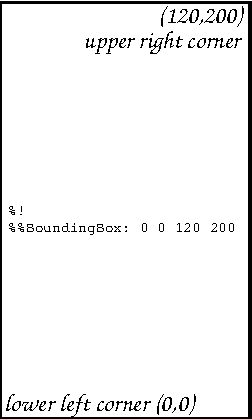
\includegraphics{figures/fig1}
% \end{figure}


\end{document}                    % DO NOT DELETE THIS LINE
%%%%%%%%%%%%%%%%%%%%%%%%%%%%%%%%%%%%%%%%%%%%%%%%%%%%%%%%%%%%%%%%%%%%%%%%%%%%%%
